\section{Question and prior work}
This follow-up asks whether current-frame conditioning improves critical pedestrian matching beyond an input-independent gate when inherited checkpoints, adaptation updates, module shapes, sampling, and inference paths are matched. It tests a bounded coefficient residual in the existing detector. Limiting departures from its learned static mixture is a design motivation. The falsifiable hypothesis is a conditioning advantage under that declared bound; both arms are bounded, so the experiment cannot establish a benefit of bounding itself. Improvement is not a completion requirement.

The completed predecessor reported mixed gate results and no stable efficacy~\cite{Wu2026CriticalMiss}. In its A2/seed1/clean comparison, pedestrian hits increased from 1,000 to 1,007 of 2,923 observations, while joint-VRU AnyMiss retained the same 288 failed identities among 307 joint-target frames. That saved-count study could not identify which individual annotations changed match status. It already included a same-shape constant-descriptor A3 control. The present direct dynamic--constant comparison tightens common pooling and execution paths under the bounded formula, while saving exact target turnover. Its smaller four-log panel and newly computed outputs are a separate experiment, not a repair or rerun of the earlier matrix, and capacity matching itself is not a new contribution.

BEVFormer builds BEV representations from camera views through spatial cross-attention and historical BEV through temporal self-attention~\cite{Li2022BEVFormer}. Its official transformer passes the encoder BEV embedding to the detection decoder~\cite{BEVFormerCode}. Our current-frame camera/LiDAR customization disables temporal history and adds LiDAR processing, so it is BEVFormer-derived rather than a reproduction of the original system. Conditional modulation and neutral residual initialization are established design ideas: FiLM conditions feature-wise affine transformations~\cite{Perez2018FiLM}, while ReZero introduces initially zero residual weights~\cite{Bachlechner2021ReZero}. Neither provides evidence for this detector's critical-miss behavior. The earlier project gate already had neutral initialization and conditioned outputs; the present changes are the bounded coefficient residual and tighter controls, without a priority claim.

\section{Architecture and gradient paths}
\begin{figure*}[t]
\centering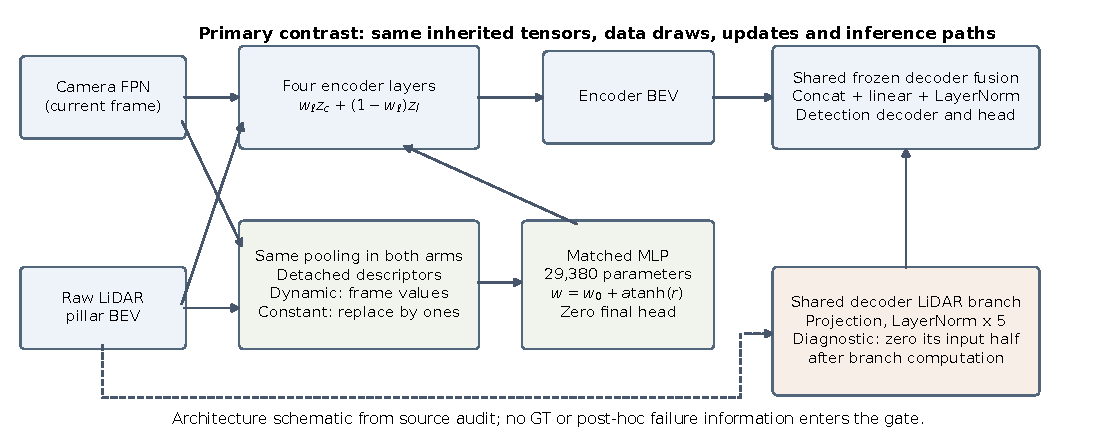
\includegraphics[width=\textwidth]{images/matched_architecture.pdf}
\caption{Matched source-level architecture. Both arms pool the actual current-frame features before retaining dynamic descriptors or replacing them with constants. The shared decoder LiDAR route is frozen; its inference masking is a separate intervention. No annotation or post-hoc failure information enters the gate.}\label{fig:architecture}
\end{figure*}
At each of four encoder layers, a scalar camera coefficient blends camera and projected-LiDAR attention outputs:
\begin{equation}
 z_\ell=w_\ell z_{\ell,c}+(1-w_\ell)z_{\ell,l}.
 \label{eq:blend}
\end{equation}
Coefficients vary by frame and layer but are shared spatially. They are not object-specific masks and receive no annotation, sample identity, prediction, or post-hoc failure information at inference. A frame containing both recovered and missed pedestrians therefore receives a common mixture at each layer; spatially selective recovery is not directly specified by this gate.

In the ordinary nonempty camera-attention branch, both attention outputs include the same query residual. Writing their remaining attention terms as $A_c,A_l$ gives $z=q+wA_c+(1-w)A_l$. The audited customized camera-attention code also has an all-camera-masks-empty fallback returning $\operatorname{dropout}(q)+q$, equal to $2q$ in evaluation for that residual input. That exception prevents treating the ordinary residual simplification as unconditional; its real-data incidence is not measured here. The shared implementation is kept fixed during this contrast; real-data incidence and impact require a separate instrumented evaluation. The general derivative using complete branch outputs remains valid:
\begin{equation}
 \frac{\partial\mathcal L}{\partial r_\ell}
 =a_\ell\operatorname{sech}^{2}(r_\ell)
 \left\langle\frac{\partial\mathcal L}{\partial z_\ell},
 z_{\ell,c}-z_{\ell,l}\right\rangle.
\end{equation}
The inner product sums spatial/channel contributions to one frame-level decision. Object-specific improvements and regressions can compete in that aggregate. The detector loss is not the discontinuous AnyMiss endpoint; observing an active gradient does not imply that the last remaining missed target in a frame will recover.

The audited implementation also routes LiDAR features to the decoder independently of Eq.~\eqref{eq:blend}. A $64\!\rightarrow\!256$ convolution and token-wise LayerNorm, scaled by five, produce the decoder LiDAR representation. It is concatenated with encoder BEV and passed through a $512\!\rightarrow\!256$ linear transformation and LayerNorm. This route is retained identically, with its parameters frozen, in both adaptation arms. The primary contrast estimates incremental conditioning \emph{conditional on this shared route}; it cannot establish gate efficacy in a detector without that route.

The source audit also finds this route in every original A0--A3 arm, under the same encoder--decoder fusion configuration and frozen adaptation guards. Its presence is therefore not, by itself, evidence of a differential architectural confound in those comparisons. The original A0 static control's four trainable logits versus the dynamic module's 29,380 parameters is a concrete parameterization difference, whereas A3 already matched the dynamic MLP's shapes. A3 skipped actual feature pooling; the new pair builds on that control, computes common pooling, and makes the shared-path condition explicit.

Gate descriptors pool detached float32 camera FPN features over views and spatial positions, average across levels, and pool raw pillar features spatially. Views and FPN levels receive equal weights, without a padding mask or object-specific pooling. Trainable projections follow detachment. Consequently, the conditioning branch does not send gradients back through descriptor construction. Detection-loss gradients still flow through the mixture and, during encoder adaptation, its attention computations. Frozen downstream weights can transmit input gradients; freezing their parameters does not sever the computation graph.

\section{Bounded gate and matched control}
Let $\alpha_\ell$ be an inherited static logit and $w_{0\ell}=\sigma(\alpha_\ell)$. Define
\begin{align}
 a_\ell&=\min\{0.1,w_{0\ell},1-w_{0\ell}\},\\
 w_\ell(x)&=w_{0\ell}+a_\ell\tanh r_\ell(x).
 \label{eq:bounded}
\end{align}
The inherited weights and amplitudes remain fixed. Equation~\eqref{eq:bounded} confines each coefficient to $[0,1]$ and its departure from the inherited mixture to at most 0.1. Neutrality reproduces the inherited learned weights, rather than resetting them to 0.5.

Camera and LiDAR descriptors are projected from 256 and 64 channels, respectively, to 64 channels each. Their concatenation passes through LayerNorm, a 128-to-64 linear layer, GELU, and a four-output linear head. The last head's weights and biases start at exactly zero. Its parameters can receive first-step gradients, whereas preceding projection and hidden-layer gradients initially vanish because the output weights are zero; they can become nonzero after the head changes. The fixed amplitude avoids multiplying two independently zero-initialized residual factors. Synthetic equality, gradient, bound, and descriptor-detachment checks verify this contract, without supplying detection evidence.

The dynamic arm uses current pooled descriptors. The constant arm computes the same pooling and replaces both descriptor vectors with ones before the same projections. Both start with the same trainable tensors, execute the same operation shapes, and contain 29,380 gate parameters and 41,952,875 total model parameters. This controls nominal parameterization and inference graph. It does not imply equal effective capacity, identical optimization, or exactly equal measured runtime. The constant arm can learn an input-independent mixture. An unadapted U8000 detector with a neutrally initialized gate is also evaluated. Its detector already has 8,000 inherited updates, but no new adaptation; its unequal update count excludes it from primary gate attribution.

There is no matched unbounded dynamic arm in this finite design. The comparison tests conditioning under the declared bound, not whether the bound itself improves the earlier dynamic gate. Likewise, differences between adapted arms can include encoder changes induced during training; they do not isolate instantaneous gate coefficients from learned encoder representations.

\section{Data roles, adaptation, and frozen protocol}
The dataset remains nuScenes mini~\cite{Caesar2020nuScenes}, with its historically exposed capture-log roles unchanged. F1 and F2 are the first panels in the original order having undamaged, existing U8000 initialization for every original seed. Their outer union contains 162 frames from four logs. Panel choice uses checkpoint availability, not new outcomes; it neither repairs the damaged historical matrix nor produces full-mini coverage. Each detector retains its original five-log training, one-log development, and two-log outer roles. Cross-fold training populations overlap.

The design fixes seeds 0, 1, and 2 and two adaptation arms in each fold: twelve trajectories of 600 updates, capped at 7,200 scientific optimizer updates. Each pair inherits the same fold/seed U8000 checkpoint and uses the final600 state only. No new development or outer endpoint selects a checkpoint, candidate, or training length. Batch size is one; paired arms use the same seeded repeated-permutation sampler and augmentation/dropout seeds, recording requested and actual sample identities. Actual draws are checked for agreement before the second arm updates. TF32 is disabled, without a bitwise CUDA reproducibility claim.

\begin{table}[t]
\centering
\small
\setlength{\tabcolsep}{3pt}
\caption{Fixed adaptation schedule. Learning rates are gate/encoder.}
\label{tab:adaptation}
\begin{tabular}{lrrl}
\toprule
Stage & Updates & \shortstack{Trainable\\parameters} & Learning rates\\
\midrule
Gate only & 200 & 29,380 & $10^{-4}$ / frozen\\
Gate + encoder & 400 & 3,553,604 & $10^{-4}$ / $10^{-5}$\\
\bottomrule
\end{tabular}
\end{table}

Both stages use AdamW, weight decay 0.01, gradient clipping at 35, and frozen batch-normalization behavior. Backbone, neck, LiDAR processing, detection head, and decoder parameters remain frozen. Engineering is bounded separately at three optimizer updates and 30 minutes. The single-GPU ceiling includes engineering and inference: 12 reserved GPU hours, 24 wall hours, 20 GB of new storage, and 40 minutes per training run. Failures and costs are retained; scientific attempts are not automatically retried or resumed. Protocol and implementation review by a separate AI agent in the same process precedes execution and does not constitute external replication.

All training precedes outcome evaluation. The primary view is clean outer data pooled within each seed. Fixed secondary views comprise the declared 50\% LiDAR perturbation, clean development data, and decoder-path masking. Masking zeros only the decoder LiDAR half immediately before its fusion linear layer, after the original branch has executed. Encoder LiDAR inputs remain active, so this does not create a camera-only detector. It is a same-checkpoint inference intervention, not a retrained control or causal estimate of path contribution.

\section{Endpoints and exact identity decomposition}
The custom endpoint preserves mapped ground truth having positive summed LiDAR/radar annotation points. Predictions with score at least 0.1 are processed in descending score order, with lexicographic decimal output-slot tie ordering. Each greedily matches the nearest unassigned same-class eligible annotation at strict center distance below 2 m; original annotation order resolves equal distances. Matching precedes restriction to pedestrian, bicycle, and motorcycle targets within inclusive ego-frame horizontal radius 30 m. These custom rules remain distinct from official SDK filtering and matching~\cite{nuScenesSDK}.

For frame $t$, let $U_t$ denote its critical annotations and $H_{a,t}\subseteq U_t$ the matched annotations under arm $a$. Pooled recall is $\sum_t|H_{a,t}|/\sum_t|U_t|$. AnyMiss is $\mathbf{1}\{|U_t\setminus H_{a,t}|>0\}$: at least one missed target, not necessarily all targets missed. Target-frame and all-frame denominators are reported separately. Empty-target frames have no AnyMiss event. Each seed retains per-log numerators, denominators, and equal-log descriptions; absent class support is disclosed rather than converted into a passing macro metric.

Annotation, instance, sample, scene, and log identities are saved during endpoint computation, together with matched prediction identity, slot, distance, score, and prediction-file hash. With constant arm $c$ and dynamic arm $d$,
\begin{align}
 R&=\sum_t|H_{d,t}\setminus H_{c,t}|,\qquad
 L=\sum_t|H_{c,t}\setminus H_{d,t}|,\\
 \Delta H&=R-L,\qquad \Delta F=N_{\rm new}-N_{\rm clear}.
\end{align}
These identify recovered and newly lost annotation observations, persistent matches/misses, fully recovered frames, and newly failed frames. Within-frame identity exchanges can occur even when hit counts are equal. Repeated observations of one instance are retained explicitly; run-local prediction slots are not cross-run tracking identities.

SDK mAP, NDS, pedestrian AP, and filtered class support are evaluated separately. Pooled SDK metrics use merged unique-token predictions rather than averaged fold AP. Each pooled seed combines two fold-specific detectors; per-log tables retain that heterogeneity, and the pooled result describes this collection rather than one deployed checkpoint. Saved outputs and all-range unmatched pedestrian counts at score at least 0.1 describe output burden, not official false positives or precision. No monitor is fitted, calibrated, or transferred from the earlier detector outputs.

The frozen descriptive criterion requires dynamic-minus-constant pedestrian recall of at least one percentage point in every original seed, no increase in joint AnyMiss failures, no negative equal-log pedestrian effect, and at most a 5\% increase in saved pedestrian outputs in every seed. Failure ends candidate expansion. This practical screen is not a statistical test or driving requirement.

